\documentclass[12pt]{article}
\newcommand{\VERSION}{0.0-2}
%\VignetteIndexEntry{addingToolkit}
%\VignettePackage{addingToolkit}

\usepackage{times}              % for fonts
\usepackage[]{geometry}
\usepackage{mathptm}            % for math fonts type 1
\usepackage{graphicx}           % for graphics files
\usepackage{floatflt}           % for ``floating boxes''
%%\usepackage{index}
\usepackage{relsize}            % for relative size fonts
\usepackage{amsmath}            % for amslatex stuff
\usepackage{amsfonts}           % for amsfonts
\usepackage{url}                % for \url,
\usepackage{color}
\usepackage{fancyvrb}
\usepackage{fancyhdr}
\usepackage{jvfloatstyle}       % redefine float.sty for my style. Hack


%% squeeze in stuff
\floatstyle{jvstyle}
\restylefloat{table}
\restylefloat{figure}
\renewcommand\floatpagefraction{.9}
\renewcommand\topfraction{.9}
\renewcommand\bottomfraction{.9}
\renewcommand\textfraction{.1}
\setcounter{totalnumber}{50}
\setcounter{topnumber}{50}
\setcounter{bottomnumber}{50}

%% Fill these in
\pagestyle{fancy}
\usepackage{fancyhdr}
\pagestyle{fancy}
\fancyhf{}
\fancyhead[L]{\RCode{gWidgets}}
\fancyhead[C]{}
\fancyhead[R]{\sectionmark}
\fancyfoot[L]{}
\fancyfoot[C]{- page \thepage\/ -}
\fancyfoot[R]{}
\renewcommand{\headrulewidth}{0.1pt}
\renewcommand{\footrulewidth}{0.0pt}

%% My abbreviations
\newcommand{\RCode}[1]{\texttt{#1}}
\newcommand{\RFunc}[1]{\texttt{#1()}}
\newcommand{\RPackage}[1]{\textbf{#1}}
\newcommand{\RArg}[1]{\texttt{#1=}}
\newcommand{\RListel}[1]{\texttt{\$#1}}


\newenvironment{RArgs}{\begin{list}{}{}}{\end{list}}


\usepackage{/usr/local/R/lib/R/share/texmf/Sweave}
\begin{document}
\thispagestyle{plain}
\title{Adding a toolkit to gWidgets}

\author{John Verzani, \url{gWidgetsRGtk@gmail.com}}
\maketitle

\section*{Abstract:}
This little vignette illustrates what is required to write a toolkit
for the \RPackage{gWidgets} package. Since the \RPackage{gWidgetsRGtk}
package is written this sketches out what a toolkit would possible
look like using the \RPackage{tcltk} package. Unfortunately, this
author does not know enough about the \RPackage{tcltk} package to
actually do this.

\setcounter{tocdepth}{3}
\tableofcontents

\section{Basics of gWidgets}

The gWidgets implementation is simply a set of functions that dispatch
to similarly named functions in a toolkit. That is the \RCode{glabel(...,toolkit=guiToolkit())}
function dispatches to the \RCode{.glabel(toolkit, ...)} function in the appropriate
toolkit, and the \RCode{svalue(obj,...)} method dispatches to the
\RCode{.svalue(obj@widget,obj@toolkit, ...)} function in the appropriate
toolkit. In the first case the dispatch is done by the class of the
toolkit. For the method, the dispatch is based on both the toolkit and
the class of the object, and perhaps other arguments in the signature
of the method.

As such, the basic structure of gWidgets is to set up some classes,
most notable a class \RCode{guiWidgetsToolkit} of which each toolkit
class is a subclass, and a set of methods for dispatch.


\section{An example}
As \RPackage{gWidgets} is supposed to be cross-toolkit, it would be
nice were there a toolkit implementation for the \RPackage{tcltk}
package. I know only as much about \RPackage{tcltk} as was learned
by browsing P. Dalgaard's RNews article and a quick glance the examples
provided by James Wettenhall.


The following is a start, although we quickly run into issues
that hopefully someone more knowledgeable about \RPackage{tcltk} can
resolve.


First we load the package.
\begin{Schunk}
\begin{Sinput}
> options(guiToolkit = NA)
> library(gWidgets)
> library(tcltk)
\end{Sinput}
\begin{Soutput}
Loading Tcl/Tk interface ... done
\end{Soutput}
\end{Schunk}

Now we make subclass \RCode{guiWidgetsToolkit} so that we can dispatch
on the toolkit.
\begin{Schunk}
\begin{Sinput}
> setClass("guiWidgetsToolkitTcltk", contains = "guiWidgetsToolkit", 
+     prototype = prototype(new("guiWidgetsToolkit")))
\end{Sinput}
\begin{Soutput}
[1] "guiWidgetsToolkitTcltk"
\end{Soutput}
\begin{Sinput}
> guitoolkit = new("guiWidgetsToolkitTcltk")
\end{Sinput}
\end{Schunk}

Now we make a base class for the tcltk widgets created here.
\begin{Schunk}
\begin{Sinput}
> setClass("gWidgetTcltk")
\end{Sinput}
\begin{Soutput}
[1] "gWidgetTcltk"
\end{Soutput}
\begin{Sinput}
> setClass("guiWidgetORgWidgetTcltkORtcltk")
\end{Sinput}
\begin{Soutput}
[1] "guiWidgetORgWidgetTcltkORtcltk"
\end{Soutput}
\begin{Sinput}
> setIs("guiWidget", "guiWidgetORgWidgetTcltkORtcltk")
> setIs("gWidgetTcltk", "guiWidgetORgWidgetTcltkORtcltk")
\end{Sinput}
\end{Schunk}

Finally, we promote the \RCode{tkwin} class to an S4 class and add it
to our virtual class. This would be done for all possible classes of
\RCode{tcltk} objects.

\begin{Schunk}
\begin{Sinput}
> oldclasses = c("tkwin")
> for (i in oldclasses) {
+     setOldClass(i)
+     setIs(i, "guiWidgetORgWidgetTcltkORtcltk")
+ }
\end{Sinput}
\end{Schunk}


The \RCode{gWidgetTcltk} class is a virtual class, here are two
subclasses. We create slots for the widget and the toolkit here, but
perhaps should add others.

\begin{Schunk}
\begin{Sinput}
> setClass("gComponentTcltk", representation(widget = "guiWidgetORgWidgetTcltkORtcltk", 
+     toolkit = "guiWidgetsToolkit"), contains = "gWidgetTcltk", 
+     )
\end{Sinput}
\begin{Soutput}
[1] "gComponentTcltk"
\end{Soutput}
\begin{Sinput}
> setClass("gContainerTcltk", representation(widget = "guiWidgetORgWidgetTcltkORtcltk", 
+     toolkit = "guiWidgetsToolkit"), contains = "gWidgetTcltk", 
+     )
\end{Sinput}
\begin{Soutput}
[1] "gContainerTcltk"
\end{Soutput}
\end{Schunk}

Now we define some necessary functions to implement \RFunc{gwindow} in
the toolkit. This involves defining a class, make a constructor
(\RFunc{.gwindow}) and defining some methods.

\begin{Schunk}
\begin{Sinput}
> setClass("gWindowTcltk", contains = "gContainerTcltk", prototype = prototype(new("gContainerTcltk")))
\end{Sinput}
\begin{Soutput}
[1] "gWindowTcltk"
\end{Soutput}
\end{Schunk}

This implementation of the constructor should add a handler for the
destroy event.
\begin{Schunk}
\begin{Sinput}
> setMethod(".gwindow", signature(toolkit = "guiWidgetsToolkitTcltk"), 
+     function(toolkit, title = "Window", visible = TRUE, handler = NULL, 
+         action = NULL, ...) {
+         win <- tktoplevel()
+         tktitle(win) <- title
+         obj = new("gWindowTcltk", widget = win, toolkit = toolkit)
+         return(obj)
+     })
\end{Sinput}
\begin{Soutput}
[1] ".gwindow"
\end{Soutput}
\end{Schunk}

The \RFunc{svalue} method for \RFunc{gwindow} objects is used to
retrieve and set the title of the window. 

\begin{Schunk}
\begin{Sinput}
> setMethod(".svalue", signature(toolkit = "guiWidgetsToolkitTcltk", 
+     obj = "gWindowTcltk"), function(obj, toolkit, index = NULL, 
+     drop = NULL, ..) {
+     tktitle(obj@widget)
+ })
\end{Sinput}
\begin{Soutput}
[1] ".svalue"
\end{Soutput}
\begin{Sinput}
> setMethod(".svalue<-", signature(toolkit = "guiWidgetsToolkitTcltk", 
+     obj = "gWindowTcltk"), function(obj, toolkit, index = NULL, 
+     ..., value) {
+     tktitle(obj@widget) <- value
+     return(obj)
+ })
\end{Sinput}
\begin{Soutput}
[1] ".svalue<-"
\end{Soutput}
\end{Schunk}

The \RFunc{add} method is used to add a widget to a container. This is
where we run into problems with \RPackage{tcltk} as the constructors
there require a ``parent'' container at the time of construction. As
such, we don't have both a container (\RCode{obj} below) and  widget
(\RCode{value}) needed when we add, rather we only specify how things
are packed in.

\begin{Schunk}
\begin{Sinput}
> setMethod(".add", signature(toolkit = "guiWidgetsToolkitTcltk", 
+     obj = "gWindowTcltk", value = "guiWidget"), function(obj, 
+     toolkit, value, ...) {
+     tkpack(value@widget@widget)
+ })
\end{Sinput}
\begin{Soutput}
[1] ".add"
\end{Soutput}
\end{Schunk}

The dispose method closes the window
\begin{Schunk}
\begin{Sinput}
> setMethod(".dispose", signature(toolkit = "guiWidgetsToolkitTcltk", 
+     obj = "gWindowTcltk"), function(obj, toolkit, ...) {
+     tkdestroy(obj@widget)
+ })
\end{Sinput}
\begin{Soutput}
[1] ".dispose"
\end{Soutput}
\end{Schunk}

Below we implement the basics of \RFunc{glabel}. No attempt is made to
add a click handler to this or editing or markup. For now, just
setting of text in a label.

First a class
\begin{Schunk}
\begin{Sinput}
> setClass("gLabelTcltk", contains = "gComponentTcltk", prototype = prototype(new("gComponentTcltk")))
\end{Sinput}
\begin{Soutput}
[1] "gLabelTcltk"
\end{Soutput}
\end{Schunk}


Next the constructor
\begin{Schunk}
\begin{Sinput}
> setMethod(".glabel", signature(toolkit = "guiWidgetsToolkitTcltk"), 
+     function(toolkit, text = "", markup = FALSE, editable = FALSE, 
+         handler = NULL, action = NULL, container = NULL, ...) {
+         if (is.null(container)) {
+             cat("Can't have an NULL container with tcltk")
+         }
+         if (is(container, "guiWidget")) 
+             container = container@widget
+         if (is(container, "gContainerTcltk")) 
+             container = container@widget
+         label = tklabel(container, text = text)
+         obj = new("gLabelTcltk", widget = label, toolkit = toolkit)
+         tkpack(label)
+         return(obj)
+     })
\end{Sinput}
\begin{Soutput}
[1] ".glabel"
\end{Soutput}
\end{Schunk}

The \RFunc{svalue} method returns the label text, to be honest I don't
know enough about the \RPackage{tcltk} package to write this, although
to set the text is easy.

\begin{Schunk}
\begin{Sinput}
> setMethod(".svalue", signature(toolkit = "guiWidgetsToolkitTcltk", 
+     obj = "gLabelTcltk"), function(obj, toolkit, index = NULL, 
+     drop = NULL, ..) {
+     cat("How to retrieve label text\n")
+ })
\end{Sinput}
\begin{Soutput}
[1] ".svalue"
\end{Soutput}
\begin{Sinput}
> setReplaceMethod(".svalue", signature(toolkit = "guiWidgetsToolkitTcltk", 
+     obj = "gLabelTcltk"), function(obj, toolkit, index = NULL, 
+     ..., value) {
+     tkconfigure(obj@widget, text = value)
+     return(obj)
+ })
\end{Sinput}
\begin{Soutput}
[1] ".svalue<-"
\end{Soutput}
\end{Schunk}

For the \RFunc{gbutton} implementation we show how to add a handler in
addition to implementing the \RFunc{svalue} method.

\begin{Schunk}
\begin{Sinput}
> setClass("gButtonTcltk", contains = "gComponentTcltk", prototype = prototype(new("gComponentTcltk")))
\end{Sinput}
\begin{Soutput}
[1] "gButtonTcltk"
\end{Soutput}
\end{Schunk}

As for the constructor we have:
\begin{Schunk}
\begin{Sinput}
> setMethod(".gbutton", signature(toolkit = "guiWidgetsToolkitTcltk"), 
+     function(toolkit, text = "", handler = NULL, action = NULL, 
+         container = NULL, ...) {
+         if (!is.null(container)) {
+             topwin = container@widget@widget
+         }
+         else {
+             topwin = gwindow(toolkit = toolkit)@widget
+         }
+         button = tkbutton(topwin, text = text)
+         obj = new("gButtonTcltk", widget = button, toolkit = toolkit)
+         tkpack(obj@widget)
+         if (!is.null(handler)) 
+             .addhandlerclicked(obj, toolkit, handler = handler)
+         return(obj)
+     })
\end{Sinput}
\begin{Soutput}
[1] ".gbutton"
\end{Soutput}
\end{Schunk}
In dealing with the handler, we used the private method defined below,
rather than \RFunc{addhandlerclicked} as that method is for objects of
class \RCode{guiWidget}, and not \RCode{gWidgetTcltk}. This awkwardness
can be avoided by defining a method \RCode{addhandlerclicked} for
objects of class \RCode{gWidgetTcltk} within the toolkit. For instance,

\begin{Schunk}
\begin{Sinput}
> setMethod("addhandlerclicked", signature(obj = "gWidgetTcltk"), 
+     function(obj, handler = NULL, action = NULL, ...) {
+         .addhandlerclicked(obj, obj@toolkit, handler, action, 
+             ...)
+     })
\end{Sinput}
\begin{Soutput}
[1] "addhandlerclicked"
\end{Soutput}
\end{Schunk}


Again, \RFunc{svalue} should retrieve the text, it shouldn't be hard,
but I don't know how. Below is how to set the button text.
\begin{Schunk}
\begin{Sinput}
> setReplaceMethod(".svalue", signature(toolkit = "guiWidgetsToolkitTcltk", 
+     obj = "gButtonTcltk"), function(obj, toolkit, index = NULL, 
+     ..., value) {
+     tkconfigure(obj@widget, text = value)
+     return(obj)
+ })
\end{Sinput}
\begin{Soutput}
[1] ".svalue<-"
\end{Soutput}
\end{Schunk}


This sets up a click handler for a button. The handler should have a
first argument which is a list with the object and the action value
passed in. This isn't done below, as it isn't clear to me how to do so
with just the \RFunc{tkconfigure} function.


\begin{figure}[htbp]
  \centering
  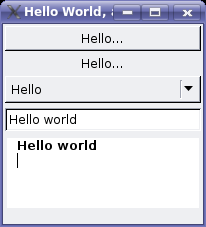
\includegraphics[width=.4\textwidth]{hello-world}
  \caption{Hello world, how are you?}
  \label{fig:hello-world}
\end{figure}



\begin{Schunk}
\begin{Sinput}
> setMethod(".addhandlerclicked", signature(toolkit = "guiWidgetsToolkitTcltk", 
+     obj = "gButtonTcltk"), function(obj, toolkit, handler, action = NULL, 
+     ...) {
+     tkconfigure(obj@widget, command = handler)
+ })
\end{Sinput}
\begin{Soutput}
[1] ".addhandlerclicked"
\end{Soutput}
\end{Schunk}

Well, that will let us make the following simple dialog
(Figure~\ref{fig:hello-world}).


\begin{Schunk}
\begin{Sinput}
> win = gwindow("Hello world", toolkit = guitoolkit)
> label = glabel("Hello world, how are you?", container = win, 
+     toolkit = guitoolkit)
> button = gbutton("Close", handler = function(h, ...) dispose(win), 
+     container = win, toolkit = guitoolkit)
\end{Sinput}
\end{Schunk}


We have to specify a container each time and for these constructors
the toolkit. If we had written a package this latter could be
avoided using the \RFunc{guiToolkit} function.


\end{document}
